\documentclass[11pt]{article}


% TODO: use polyflossia
\usepackage[english, spanish]{babel}

% font specification
\usepackage{fontspec}
% \setmainfont{TeX Gyre Pagella}
% \setmainfont[Mapping=tex-text]{TeX Gyre Pagella}
% \setmainfont[Ligatures=TeX]{TeX Gyre Pagella}

\setmainfont[Mapping=tex-text]{LinLibertineO}
\newfontfamily\ipa{LinLibertineO}

% \setsansfont[Scale=MatchLowercase]{Latin Modern Sans}
% \setsansfont[Scale=MatchLowercase]{Linux Biolinum O}
\setsansfont[Scale=MatchLowercase]{Carlito}

% consolas no es free pero tiene bold, inconsolata es al vesre
% \setmonofont[Scale=MatchLowercase]{Inconsolata}
% \setmonofont[Scale=MatchLowercase]{Consolas}
\setmonofont[Scale=MatchLowercase]{DejaVu Sans Mono}

% page sizes and margins
\usepackage{geometry}
\geometry{paper=a4paper, left=2.75cm, right=2.75cm, bottom=2.5cm, foot=2cm, top=3.5cm}
\setlength{\headheight}{14pt}

% hyperlinks in pdfs
\usepackage{hyperref}
\hypersetup{pdftitle=, pdfauthor=,pdfborder={0 0 0}, colorlinks=false, linkcolor=black, citecolor=black, filecolor=black}
\hypersetup{pdftitle={Resolución de la ecuación de transporte mediante el método de las características en el código neutrónico milonga}, pdfauthor={Ramiro Vignolo}}

% headers & footers
\usepackage{fancyhdr}
\makeatletter
\fancyhead[L]{\@docnumber-\@docrevision}
\fancyhead[C]{}
\fancyhead[R]{\thepage/\pageref{lastpage}}
\fancyfoot[L]{\includegraphics[height=10pt]{theme/logo-nasa}}
\fancyfoot[C]{\tiny{\texttt{23436d43f9bb}}}
% \fancyfoot[R]{\thepage}
\fancyfoot[R]{\includegraphics[height=10pt]{theme/logo-tecna}}
\makeatother
\renewcommand{\headrulewidth}{0.4pt}
% \renewcommand{\footrulewidth}{0.4pt}
\pagestyle{fancy}

% biblatex
\usepackage{csquotes}     % this package is needed for \blx@bibinit below (sic)
\usepackage[backend=biber,sorting=none]{biblatex}    
\addbibresource{bibliografia.bib}
% initialize macros so \bibstring can be used to show some fields (needs csquotes)
\makeatletter
\blx@bibinit
\makeatother

% Font style for figures' and tables' captions
\usepackage[small,bf,up]{caption}
\renewcommand{\captionfont}{\scriptsize\sf}

% things
\usepackage{lastpage}
\usepackage{graphicx}
\usepackage{amsmath}
\usepackage{amssymb}
\usepackage{rotating}
\usepackage{tabularx}
\usepackage[table]{xcolor}
\usepackage{eso-pic}
\usepackage{subfig}
\usepackage{listings}
\usepackage{xltxtra}
\usepackage{siunitx}


\usepackage{booktabs}
\usepackage{lscape}
\usepackage{breqn}

% vectors done right
\renewcommand{\vec}[1]{\ensuremath\mathbf{#1}}

% textpos para poner bloques de texto en posiciones absolutas
\usepackage[absolute]{textpos}
\setlength{\TPHorizModule}{2.5mm}
\setlength{\TPVertModule}{\TPHorizModule}
\textblockorigin{0mm}{\paperheight}


\makeatletter 
% these fields are defined as TeX macros so they can be used as such,
% i.e.  in the fancyhdr package
\def\affiliation#1{\def\@affiliation{#1}}

\newcommand{\fielddesc}[1]{\textsf{\footnotesize{#1}}}

\def\maketitle{%
\thispagestyle{empty}

\newlength{\coff}
\setlength{\coff}{0.3cm}

% --- title -------------------------------------------------------
\null
\vspace{0.5cm plus 0.5cm minus 0.5cm}

\begin{center}
\begin{minipage}{0.8\linewidth}
\begin{center}
\Large{\textbf{\textsc{\@title}}}

\vspace{0.75cm plus 0.2cm minus 0.1cm}

\large{\@author}

\vspace{1.25cm plus 0.25cm minus 0.25cm}

\small{\@affiliation}
\vspace{1cm plus 0.2cm minus 0.2cm}

\end{center}
\end{minipage}
\end{center}

}

\makeatother

\begin{document}


\title{Resolución de la ecuación de transporte mediante el método de las características en el código neutrónico milonga}
\author{Vignolo, R.$^{1}$}
\affiliation{%
$^1$TECNA Estudios y Proyectos de Ingeniería S.A.\\
Encarnaci\'on Ezcurra 365, C1107CLA~Buenos Aires, Argentina\\
\url{rvignolo@tecna.com}\\
}


\maketitle


\begin{abstract}
\noindent
Milonga es un código de cálculo neutrónico que resuelve la ecuación de transporte estacionaria y multigrupo tanto mediante la formulación de difusión como la de ordenadas discretas ($S_N$) sobre mallas no estructuradas (aunque mallas simples estructuradas son también soportadas). Ambas formulaciones pueden ser resueltas sobre esquemas de volúmenes o elementos finitos. Milonga nació como parte del desarrollo de una tesis de doctorado de ingeniería nuclear y, al ser \emph{software} libre, permite que distintos colaboradores participen activamente en su desarrollo y no ser, como Stamm'ler decía, usuarios que ``\emph{will never understand the programs they are to use and, as computer slaves, consider them as black boxes, blindy trusting their results''} (Stamm'ler et al., 1983). La implementación del método de las características (MoC) incorpora dentro de milonga una formulación capaz de ser aplicada en cálculos de celda, rellenando la etapa faltante en cálculos de producción: celda (MoC), celda-núcleo ($S_N$) y núcleo (difusión). En esta primera instancia del desarrollo de formulaciones de celda, MoC fue seleccionado por sobre el método de las probabilidades de colisión debido a que éste no produce matrices densas, por lo que es posible resolver problemas con mayor cantidad de regiones. En este contexto, se desarrolló un eficiente algoritmo de \emph{ray tracing} sobre mallas no estructuradas y estructuradas y un \emph{solver} de potencias no lineal que, mediante la resolución de la ecuación de transporte en cada \emph{track}, permite obtener el flujo escalar en cada región y grupo de energía. En este trabajo se discute acerca de la implementación del método, los resultados preliminares obtenidos y las futuras mejoras e incorporaciones.
\end{abstract}

\vfill

\begin{center}
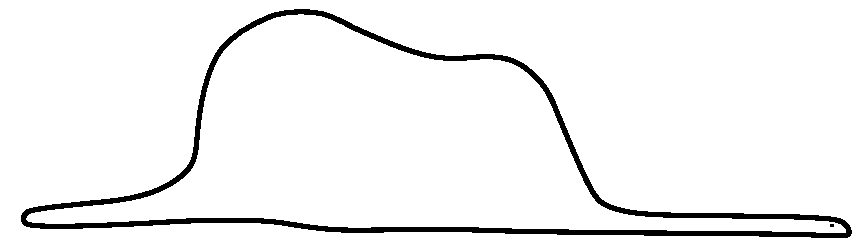
\includegraphics[width=5cm]{vibora-blanca-sola.pdf}
\end{center}

\vfill

\begin{center}
\begin{small}
XLIII Reunión Anual de la Asociación Argentina de Tecnología Nuclear\\
Buenos Aires, Noviembre 2016
\end{small}
\end{center}

\addtolength{\textheight}{-2cm}


\end{document}

